\documentclass[17pt]{beamer}
\usepackage{amsmath}
\usepackage{framed}
\definecolor{Blue}{RGB}{0.16,0.32,0.75}
\setbeamercolor{structure}{fg=blue}
\usepackage{beamerthemesplit}




\definecolor{blue}{rgb}{0.16,0.32,0.75}
\setbeamercolor{structure}{fg=blue}
\author[FOSSEE]{}
\institute[IIT Bombay]{}
\date[]{}
% \setbeamercovered{transparent}

% theme split
\usepackage{verbatim}
\newenvironment{colorverbatim}[1][]%
{%
\color{blue}
\verbatim
}%
{%
\endverbatim
}%

\usepackage{mathpazo,courier,euler}
\usepackage{listings}
\lstset{language=sh,
    basicstyle=\ttfamily\bfseries,
  showstringspaces=false,
  keywordstyle=\color{black}\bfseries}

% logo
\logo{
\includegraphics[height=1.30 cm]{St-logo.png}}
\logo{
\includegraphics[height=1.30 cm]{fossee-logo.png}

\hspace{7.5cm}

\includegraphics[scale=0.3]{fossee-logo.png}\\
\hspace{281pt}

\includegraphics[scale=0.08]{St-logo.png}}


\newcounter{saveenumi}
\newcommand{\seti}{\setcounter{saveenumi}{\value{enumi}}}
\newcommand{\conti}{\setcounter{enumi}{\value{saveenumi}}}

\begin{document}
% sf family, bold font
\sffamily \bfseries
%\LARGE
\title
[Python for Scientific Computing]
%\hspace{0.5cm}
%\insertframenumber/\inserttotalframenumber]
{\large Other types of plots}
\author
[FOSSEE, IIT Bombay]
{{\small Spoken Tutorial Project \\ http://spoken-tutorial.org \\ National Mission on Education  through ICT  \\ http://sakshat.ac.in } \\
{\small Script: Thirumalesh H S}\\
{\small Narrator: Kiran Kishore}\\
{\small IIT Bombay}\\
{\small  26 October 2015}}

% slide 1
\begin{frame}
   \titlepage
\end{frame}
%%%%%%%%%%%%%%%%%%%%%%%%%%%%%%%%%%%%%%%%%%%%%%%%%%%%%%%%%%%%%%%%%%%%%%%%%%%%%%%%
\begin{frame}
\frametitle{Objectives}

  At the end of this tutorial, you will be able to -\pause

\begin{itemize}
\item Create pie charts\pause
\item Create bar charts\pause
\item Find more information on matplotlib
\end{itemize}
\end{frame}
%%%%%%%%%%%%%%%%%%%%%%%%%%%%%%%%%%%%%%%%%%%%%%%%%%%%%%%%%%%%%%%%%%%%%%%%%%%%%%%%
\begin{frame}
\frametitle{System Specifications}\pause
\begin{itemize}
\item Ubuntu Linux 14.04\pause
\item \texttt{Python 2.7.6} \pause
\item \texttt{IPython 4.0.0}
\end{itemize}
\end{frame}
%%%%%%%%%%%%%%%%%%%%%%%%%%%%%%%%%%%%%%%%%%%%%%%%%%%%%%%%%%%%%%%%%%%%%%%%%%%%%%%%
\begin{frame}
\frametitle{Pre-requisites}
To practise this tutorial, you should know how to
\begin{itemize}
\item run basic Python commands on the ipython console\pause
\item load data from files and plot data.\pause
\end{itemize}
If not, see the pre-requisite Python tutorials on
{\color{blue}http://spoken-tutorial.org}
\end{frame}
%%%%%%%%%%%%%%%%%%%%%%%%%%%%%%%%%%%%%%%%%%%%%%%%%%%%%%%%%%%%%%%%%%%%%%%%%%%%%%%%
\begin{frame}
\frametitle{Pie chart}
A pie chart is a circular chart divided into sectors, illustrating proportion.
\end{frame}
%%%%%%%%%%%%%%%%%%%%%%%%%%%%%%%%%%%%%%%%%%%%%%%%%%%%%%%%%%%%%%%%%%%%%%%%%%%%%%%%
\begin{frame}[fragile]
\frametitle{pie() function}
\begin{itemize}
\item Syntax : \texttt{pie(values,labels=labels)}\pause
\begin{itemize}
\item values, the data to be plotted\pause
\item labels, the label for each wedge in the pie chart
\end{itemize}
\end{itemize}
\end{frame}
%%%%%%%%%%%%%%%%%%%%%%%%%%%%%%%%%%%%%%%%%%%%%%%%%%%%%%%%%%%%%%%%%%%%%%%%%%%%%%%%
\begin{frame}[fragile]
\frametitle{Exercise 1: Pie chart}
Plot a pie chart representing the profit percentage of company A. Use the data from the file company-a-data.txt.
\end{frame}
%%%%%%%%%%%%%%%%%%%%%%%%%%%%%%%%%%%%%%%%%%%%%%%%%%%%%%%%%%%%%%%%%%%%%%%%%%%%%%%%
\begin{frame}[fragile]
\frametitle{Exercise 2: Pie chart}
\begin{itemize}
\item Plot a pie chart with the same data with colors for each wedges as white, red,
magenta, yellow, blue, green, cyan, yellow, magenta, and blue.\pause
\item \textbf{Clue} - try \texttt{pie?} in your \texttt{ipython} interpreter
\end{itemize}
\end{frame}
%%%%%%%%%%%%%%%%%%%%%%%%%%%%%%%%%%%%%%%%%%%%%%%%%%%%%%%%%%%%%%%%%%%%%%%%%%%%%%%%
\begin{frame}
\frametitle{Bar chart}
A bar chart is a chart with rectangular bars with lengths proportional to the values that they represent.
\end{frame}
%%%%%%%%%%%%%%%%%%%%%%%%%%%%%%%%%%%%%%%%%%%%%%%%%%%%%%%%%%%%%%%%%%%%%%%%%%%%%%%%
\begin{frame}[fragile]
\frametitle{bar() function}
\begin{itemize}
\item Syntax : \texttt{bar(x, y)}\pause
\begin{itemize}
\item x - a sequence of data\pause
\item y - a sequence of data, the same length of x
\end{itemize}
\end{itemize}
\end{frame}
%%%%%%%%%%%%%%%%%%%%%%%%%%%%%%%%%%%%%%%%%%%%%%%%%%%%%%%%%%%%%%%%%%%%%%%%%%%%%%%%
\begin{frame}[fragile]
\frametitle{Exercise 3: Bar chart}
Plot a bar chart representing the profit percentage of company A. Use the data from the file company-a-data.txt.
\end{frame}
%%%%%%%%%%%%%%%%%%%%%%%%%%%%%%%%%%%%%%%%%%%%%%%%%%%%%%%%%%%%%%%%%%%%%%%%%%%%%%%%
\begin{frame}
\frametitle{Exercise 4: Bar chart}
\begin{itemize}
\item Plot a bar chart which is not filled and which is hatched with
45$^o$ slanting lines as shown in the image.
\item The data for the chart may be obtained from the file `company-a-data.txt.'
\end{itemize}
\end{frame}
%%%%%%%%%%%%%%%%%%%%%%%%%%%%%%%%%%%%%%%%%%%%%%%%%%%%%%%%%%%%%%%%%%%%%%%%%%%%%%%%
\begin{frame}
\frametitle{Exercise 5: Bar chart}
\begin{center}
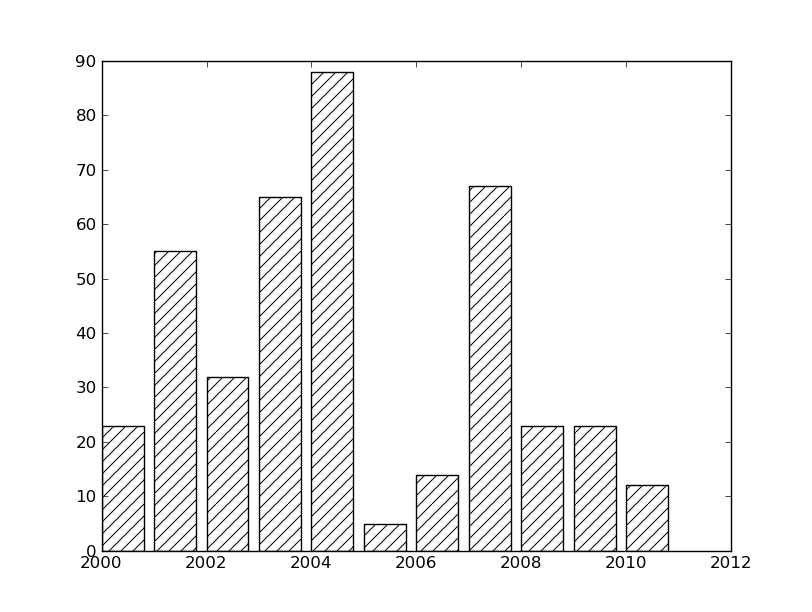
\includegraphics[scale=0.3]{bar-chart-hatch.png}
\end{center}
\begin{itemize}
\item {Clue} - try \texttt{bar?} in \texttt{ipython} interpreter
\end{itemize}
\end{frame}
%%%%%%%%%%%%%%%%%%%%%%%%%%%%%%%%%%%%%%%%%%%%%%%%%%%%%%%%%%%%%%%%%%%%%%%%%%%%%%%%
\begin{frame}
\frametitle{Getting help on matplotlib}
\begin{itemize}
\item Help about \texttt{matplotlib} can be obtained from 
\begin{itemize}
\item \url{matplotlib.sourceforge.net/contents.html}\pause
\end{itemize}
\item More plots can be seen at
\begin{itemize}
\item \url{matplotlib.sourceforge.net/users/screenshots.html}\pause
\item \url{matplotlib.sourceforge.net/gallery.html}
\end{itemize}
\end{itemize}
\end{frame}
%%%%%%%%%%%%%%%%%%%%%%%%%%%%%%%%%%%%%%%%%%%%%%%%%%%%%%%%%%%%%%%%%%%%%%%%%%%%%%%%
\begin{frame}
\frametitle{Summary}
In this tutorial, we learnt to -\pause
\begin{itemize}
\item Plot a pie chart using \texttt{pie()} function\pause
\item Plot a bar chart using \texttt{bar()} function\pause
\item Access the \texttt{matplotlib} online help.
\end{itemize}
\end{frame}
%%%%%%%%%%%%%%%%%%%%%%%%%%%%%%%%%%%%%%%%%%%%%%%%%%%%%%%%%%%%%%%%%%%%%%%%%%%%%%%%
\begin{frame}
\frametitle{Evaluation}
\begin{enumerate}
\conti
\item What statement can be issued to generate a bar chart with vertical
line hatching.
\begin{itemize}
\item bar(x, y, color='w', hatch='/')
\item bar(x, y, fill=False, hatch='//')
\item bar(x, y, fill=False, hatch='$|$')
\item bar(x, y, color='w', hatch='$\backslash$')
\end{itemize}
\end{enumerate}
\end{frame}
%%%%%%%%%%%%%%%%%%%%%%%%%%%%%%%%%%%%%%%%%%%%%%%%%%%%%%%%%%%%%%%%%%%%%%%%%%%%%%%%
\begin{frame}
\frametitle{Solutions}
\begin{enumerate}
\item bar(x, y, fill=False, hatch='$|$')
\end{enumerate}
\end{frame}
%%%%%%%%%%%%%%%%%%%%%%%%%%%%%%%%%%%%%%%%%%%%%%%%%%%%%%%%%%%%%%%%%%%%%%%%%%%%%%%%
\begin{frame}
\frametitle{Forum to answer questions}
\begin{itemize}
\item Do you have questions in THIS Spoken Tutorial?
\item Choose the minute and second where you have the question.
\item Explain your question briefly.
\item Someone from the FOSSEE team will answer them. Please visit 
\end{itemize}
\begin{center}
{\color{blue}{http://forums.spoken-tutorial.org/}}
 \end{center} 
\end{frame}
%%%%%%%%%%%%%%%%%%%%%%%%%%%%%%%%%%%%%%%%%%%%%%%%%%%%%%%%%%%%%%%%%%%%%%%%%%%%%%%%
\begin{frame}
\frametitle{Forum to answer questions}
\begin{itemize}
\item Questions not related to the Spoken Tutorial?
\item Do you have general / technical questions on the Software?
\item Please visit the FOSSEE Forum
\begin{center}
{\color{blue}{http://forums.fossee.in/}}
 \end{center}
\item Choose the Software and post your question.
\end{itemize}
\end{frame}
%%%%%%%%%%%%%%%%%%%%%%%%%%%%%%%%%%%%%%%%%%%%%%%%%%%%%%%%%%%%%%%%%%%%%%%%%%%%%%%%
\begin{frame}
\frametitle{Textbook Companion Project}
\begin{itemize}
\item The FOSSEE team coordinates coding of solved examples of popular
  books 
\item We give honorarium and certificate to those who do this
\end{itemize}
For more details, please visit this site:
\begin{center}
{\color{blue}{http://tbc-python.fossee.in/}}
\end{center}
\end{frame}
%%%%%%%%%%%%%%%%%%%%%%%%%%%%%%%%%%%%%%%%%%%%%%%%%%%%%%%%%%%%%%%%%%%%%%%%%%%%%%%%
\begin{frame}
\frametitle{Acknowledgements}
\begin{itemize}
\item Spoken Tutorial Project is a part of the Talk to a Teacher  project 
\item It is supported by the National Mission on Education through  ICT, MHRD, Government of India 
\item More information on this Mission is available at: \\{\color{blue}\url{http://spoken-tutorial.org/NMEICT-Intro}}
\end{itemize}
\end{frame}
%%%%%%%%%%%%%%%%%%%%%%%%%%%%%%%%%%%%%%%%%%%%%%%%%%%%%%%%%%%%%%%%%%%%%%%%%%%%%%%%
\begin{frame}

  \begin{block}{}
  \begin{center}
  \textcolor{blue}{\Large THANK YOU!} 
  \end{center}
  \end{block}
\begin{block}{}
  \begin{center}
    For more Information, visit our website\\
    {http://fossee.in/}
  \end{center}  
  \end{block}
\end{frame}

\end{document}
